\chapter{Paper 7}\label{sc:p7}
\textbf{\Large An 8-bit 60-MS/s 8.5mW Differential Comparator-Based Switched-Capacitor
  Pipelined ADC in 90nm CMOS Technology}\\
\indent Carsten Wulff and Trond Ytterdal\\
\indent Submitted to Journal of Solid State Circuits\\
\renewcommand\myfigname{cbscfig:}
\renewcommand\myeqname{cbsceq:}

\newcommand{\myinlref}{\reg{inl_nocal}, \reg{inl_offcal} and
  \reg{inl_gacal} }

\newcommand{\myinl}{
\begin{figure}[htbp]
\centerline{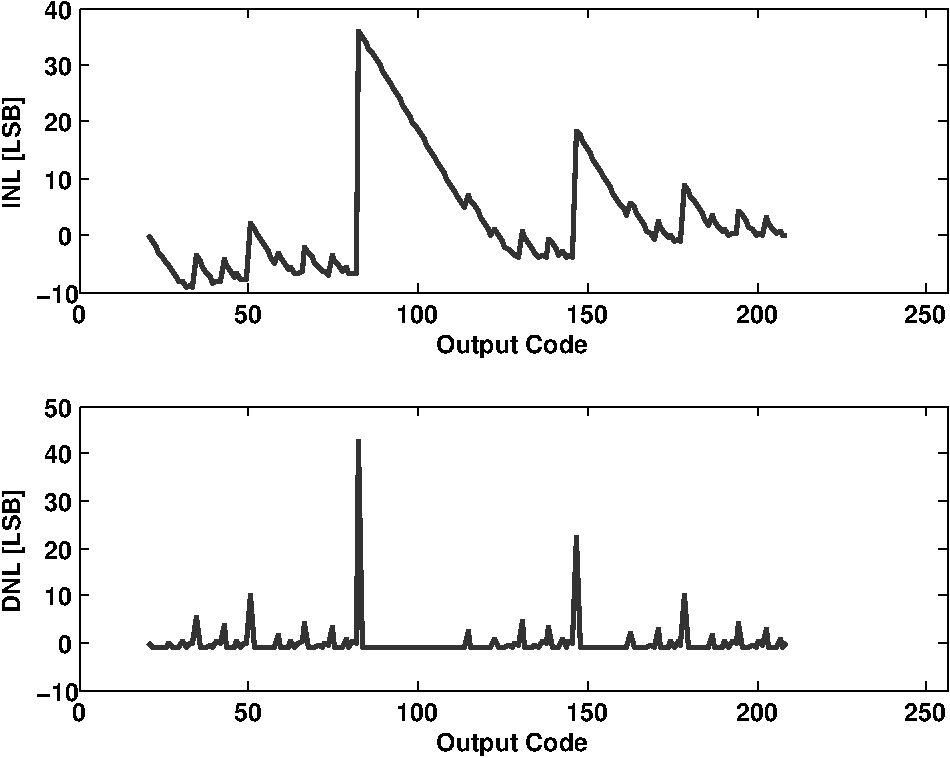
\includegraphics[width=\myfigwidth]{graphics/inl_nocal}}
\label{cbscfig:inl_nocal} 
\label{cbscfig:inl_cal}
 \caption{No calibration, default values set before before
   production}
\end{figure} 
\begin{figure}[htbp]
\centerline{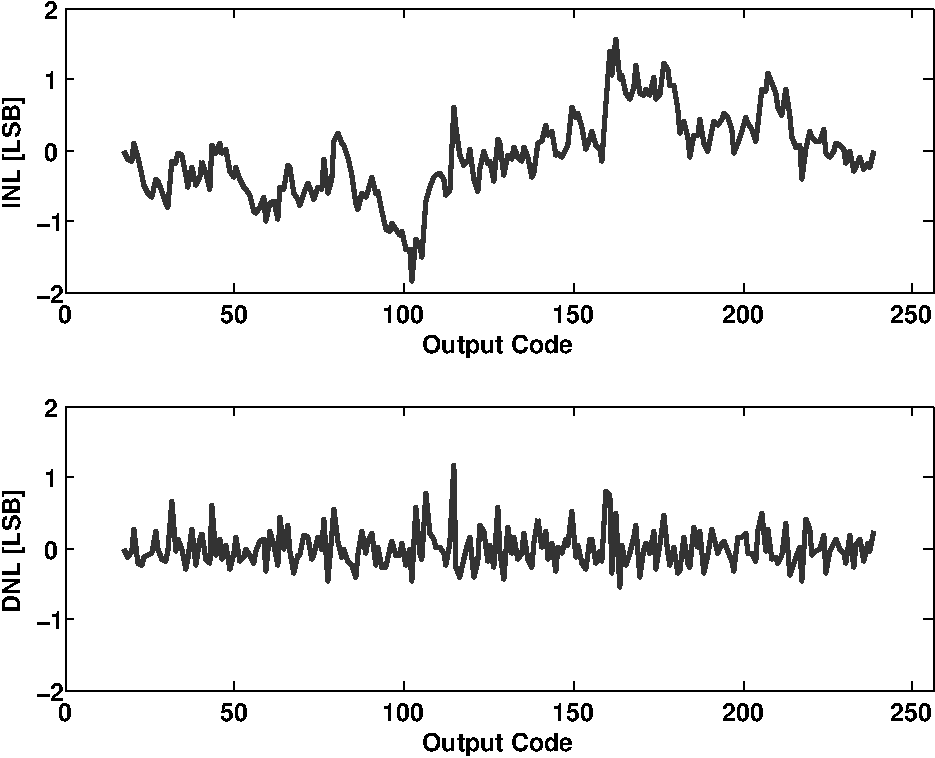
\includegraphics[width=\myfigwidth]{graphics/inl_offcal}}
\label{cbscfig:inl_offcal}
\caption{Deterministic calibration of comparator
 thresholds with current fixed}
\end{figure}
\begin{figure}[htbp]
\centerline{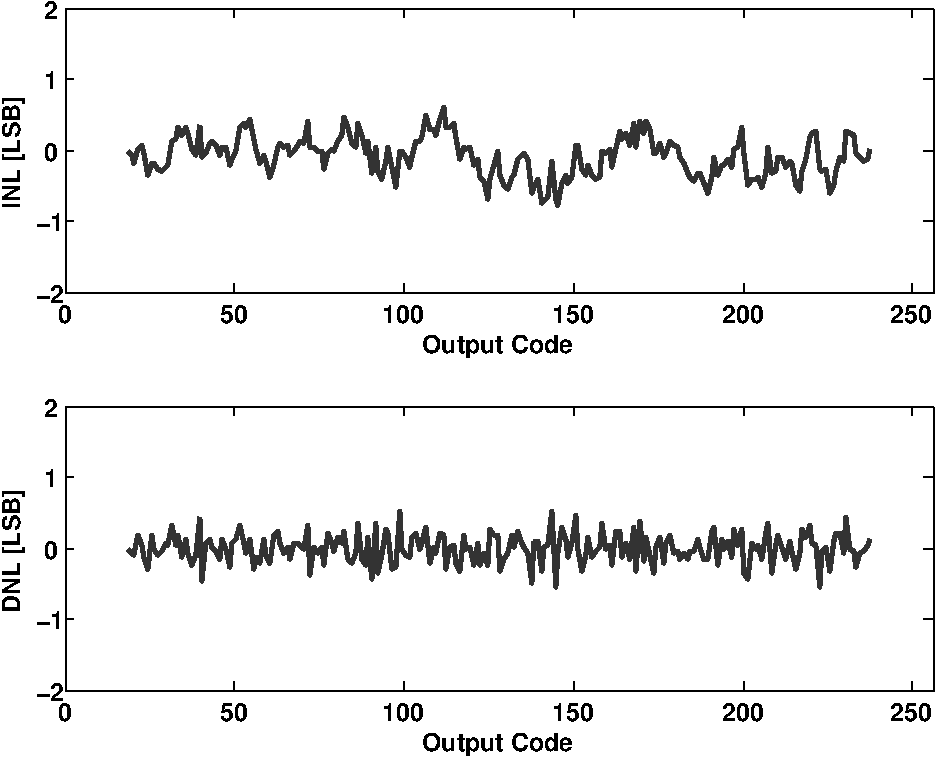
\includegraphics[width=\myfigwidth]{graphics/inl_optcal}}
 \caption{Non-deterministic calibration of positive and negative current plus
 comparator threshold using a genetic
 algorithm.}
\label{cbscfig:inl_gacal}
 \end{figure}
}

\section*{Errata}
\begin{itemize}
\item INL \& DNL: It was later discovered that the INL and DNL was
  calculated with far to few points, and as a result, contained
  significant noise. With the current number of points there is a 95\%
  confidence level of a DNL error of 0.4LSB. 
\end{itemize}




%------------------------------------------------------------------------
%\section{Abstract}
\begin{abstract}
%------------------------------------------------------------------------
We present the first differential \textit{comparator-based switched-capacitor}
(CBSC) pipelined ADC. The switched-capacitor \textit{multiplying 
digital-to-analog converter} (MDAC)
use current sources and a comparator to do charge transfer. Continuous
time bootstrapped switches are used in the first stage to reduce signal dependent switch
resistance. A simple calibration algorithm correct for
comparator delay variation due to manufacturing. Calibration reduces
ramp overshoot, which dominate the non-linearity in CBSC ADCs. The ADC is produced in a 90nm
low-power CMOS technology. The ADC core is 0.85mm x 0.35mm, with a
1.2V supply for the core and 1.8V for the input switches. The ADC
has an effective number of bits (ENOB) of 7.05-bit, and a power
dissipation of 8.5mW at 60MS/s. \\ 


%Carsten Wulff, carsten@wulff.no, Address: Radyrvegen 3, 7560
%  Vikhamer, NO-7560 Norway. Phone: +47 932 007 14.\\
%Trond Ytterdal, ytterdal@iet.ntnu.no, Address: Department of
%  electronics and telecommunication, Norwegian University of Science
%  and Technology, NO-7491 Trondheim.

\end{abstract}

\begin{IEEEkeywords}
%\paragraph{Keywords}
 Comparator-based switched-capacitor circuits, analog-to-digital,
 pipelined analog-to-digital converters
\end{IEEEkeywords}
%-------------------------------------------------------
\section{Introduction}
%-------------------------------------------------------
\IEEEPARstart{D}{ownscaling} of CMOS technology continue to challenge the analog
designer. Reduced power supply, due to reliability concerns
\cite{iwai99}, and reduced
transistor output resistance, due to shorter channels
\cite{annema05}, lead to low headroom and low intrinsic
gain. As a consequence, high-gain
operational amplifiers (opamp)|the key component in most
switched-capacitor circuits|is hard to design in nano-scale
technologies.

 Techniques like correlated level shifting
\cite{gregoire08}, open-loop residue amplifiers \cite{murmann03}, gain calibration \cite{hernes07,mcneill05}, and
comparator-based switched-capacitor circuits (CBSC)  \cite{sepke06} have been
developed to either make the opamp easier to design, or replace the
opamp completely. 

Introduced in
\cite{sepke06} CBSC is a completely new approach to switched-capacitor
circuits. It replaces the opamp with a comparator and a current
source; to demonstrate the technique a prototype 10-bit 8-MS/s 
2.5-mW pipelined ADC was presented at ISSCC 2006 \cite{sepke06}. A
year later a 200-MS/s 8-bit 8.5-mW Zero-Crossing-Based pipelined ADC,
which replaced the comparator with a zero-crossing detector,
was presented \cite{brooks07}. These implementations were
 detailed in
\cite{fiorenza06} and \cite{brooks07a}.

 Both prototypes were single ended
implementations. Single ended ADCs suffer under greater sensitivity to
power supply noise and lower signal swings compared to a differential
ADC. 

We present a differential implementation of a
CBSC ADC, and to the best of our knowledge, it is the first silicon
proven differential CBSC. Although, simulation
results of a pseudo-differential 
CBSC sigma-delta is detailed in
\cite{prelog07}.

The paper is organized as follows:
Section \ref{cbscopamp} summarize opamp based switched-capacitor
circuits. Section \ref{cbsccbsc} explain the CBSC circuits and detail a
model of the output voltage of a CBSC MDAC. The circuit implementation
is explained in Section \ref{cbsccircuit}. Calibration of the ADC is
presented in Section \ref{cbsccalibration} and in Section
\ref{cbscresults} we present
the measurement results.



%-------------------------------------------------------
\section{Opamp based switched-capacitor circuits} \label{cbscopamp}
%-------------------------------------------------------
\textit{Switched-capacitor} (SC) circuits are prevalent in pipelined ADCs
because of their robustness and accuracy. Doing
arithmetic operations like summation, subtraction, and amplification
is possible in SC circuit with high accuracy. 
The 
accuracy of SC circuits is limited by capacitor matching, which can be
accurately set in integrated circuits (on the order of 0.1 percent
\cite[page 185]{johns}).  

%Fig. \ref{cbscfig:opsc_vs_cbsc} shows a comparison between opamp based
%SC and comparator-based SC. 
SC circuits are usually designed with an opamp feedback loop as shown in
Fig. \ref{cbscfig:sccmult}. Most SC circuits have two clock phases,
sampling and charge transfer. 

Fig. \ref{cbscfig:sccmult} is an  
amplifier where the input is sampled in phase $p_1$, and charge is
transferred from
$C_1$ to $C_2$ in $p_2$ by forcing $V_x$ to
ground. If we assume the opamp has infinite gain the discrete time transfer
function for Fig. \ref{cbscfig:sccmult} is a  delayed
amplification of the input signal
\eqn{
H_0(z) = \frac{C_1+C_2}{C_2} z^{-1}
}
 where the gain is determined by the capacitance
ratio. 

With finite gain in the opamp the transfer function is
\eqn{
H_1(z) = H_0(z) \times\frac{1}{1+(C_1/C_2+1)/A}
}
where $A$ is the DC gain of the opamp.  For the remainder of this work we assume $C_1 = C_2$, so the
amplifier has a gain of two.

Finite gain in the
opamp reduce the gain of the SC amplifier.
Normally a gain error is not a significant problem, but in pipelined
ADCs a gain error in the MDAC cause static non-linearities, which 
reduce the accuracy of the converter.  

%In technologies 
%like 0.35$\mu$m CMOS  a high DC gain requirement pose
%few problems. It is trivial to make two
%stage amplifiers with enough gain for high accuracy systems. And if a
%two stage amplifier does not have enough gain, one can use
%cascoding, or gain boosting.

% As the
%CMOS technology scales, however, it is increasingly
%difficult to achieve a high DC gain. The supply voltage due to
%the decreased output resistance of nano-scale transistors and reduced
%headroom. 

%Speed can be
%traded against gain by increasing channel
%lengths, but this often an undesirable trade-of. 

% \begin{figure}[htbp]
% \centerline{ 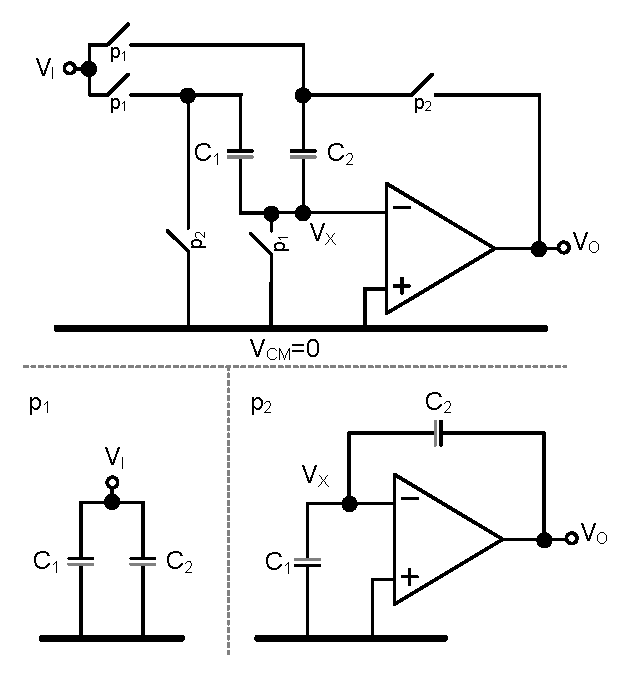
\includegraphics[width=\myfigwidthb]{graphics/sccmult}}
%   \caption{Switched-capacitor amplifier using an operational amplifier}
%   \label{cbscfig:sccmult}
% \end{figure}

\section{Comparator-based switched-capacitor circuits}\label{cbsccbsc}
It does not matter how a SC circuit arrive at the output
voltage. What matters is that the output voltage is correct when the 
next stage samples, which usually is at the end of charge transfer. 

Instead of an opamp a current source and a comparator can
be used to do charge transfer \cite{sepke06}. An opamp forces the virtual ground condition
while CBSC charge the output with a current source and detect when
virtual ground is reached. An example of a single ended CBSC is shown in
Fig. \ref{cbscfig:sc-cbsc}, only charge transfer phase is shown, sampling
phase is equivalent to opamp based SC.

 First, the output is reset to
the lowest voltage in the system (usually the negative supply
(VSS)). This ensures that $V_X$ start 
below the virtual ground (common mode). The current source is turned
on at the start of
reset and use reset to settle.
 When reset ends the current
source charge the output capacitance. The voltage at 
$V_o$ and $V_X$ rise until the comparator detect virtual ground ($V_X
 = V_{CM}=0$). Due to the comparator delay it takes a moment for the
 current source to turn off, which results in a overshoot. 

The
 overshoot can be corrected in several ways. One way is using two
 ramps \cite{sepke06}, one fast and
 one slow, the fast ramp does an estimate of the output voltage, while
 a slow ramp in the opposite direction discharge the 
 overshoot. Another is to change the threshold of the
 comparator to compensate for the overshoot \cite{brooks07}. An
 overshoot can be completely cancelled if the ramp is constant. 

A
 fundamental difference between opamp based SC and CBSC is that opamp based SC settle during charge
transfer, CBSC never settle. The current from the current source is
fully on until it is turned off. In an opamp based SC all currents in
capacitors and switches (outside of the opamp) go asymptotically to
zero as the opamp settle. In CBSC the current in capacitors and
switches are in one of two states, constant or zero, and they are
only zero when the final value has been determined. As a result, switch resistance cause offset and a
non-linearity (switches have signal dependent resistance) \cite{fiorenza06,brooks07a}. But effects
can be minimized by splitting the current source \cite{brooks07a}, or
reducing switch resistance. Reduced current helps, but the current
in CBSC is
proportional to sampling frequency, so high speed require high current.

The noise properties of
comparator-based and zero-crossing-based converters has been
exhaustively covered by \cite{sepke06th} and \cite{chow07} and
will not be discussed in this work. 

A analytical model of the MDAC output voltage is
presented in the next section.

\begin{figure*}[htbp]
 \begin{centering}
 \subfigure[Switched-capacitor amplifier using an operational amplifier.]{\label{cbscfig:sccmult} 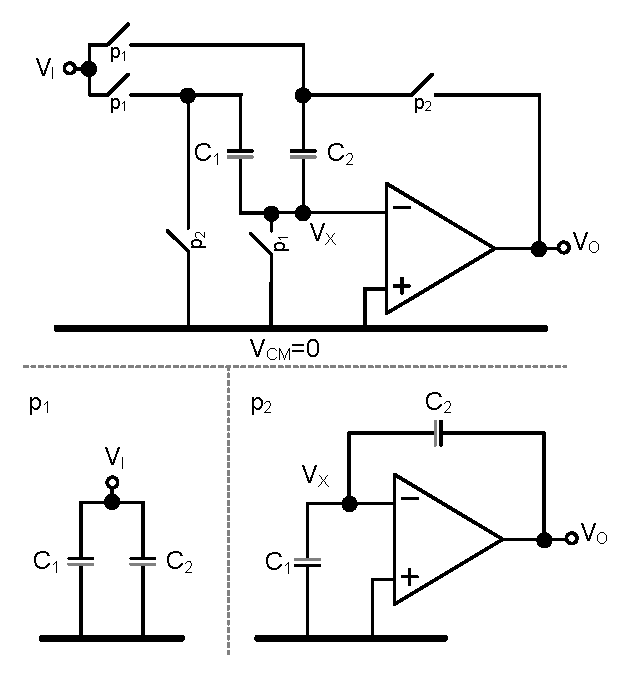
\includegraphics[width=\myfigwidthb]{graphics/sccmult}}
 \subfigure[Comparator-based switched-capacitor circuit.]{\label{cbscfig:sc-cbsc}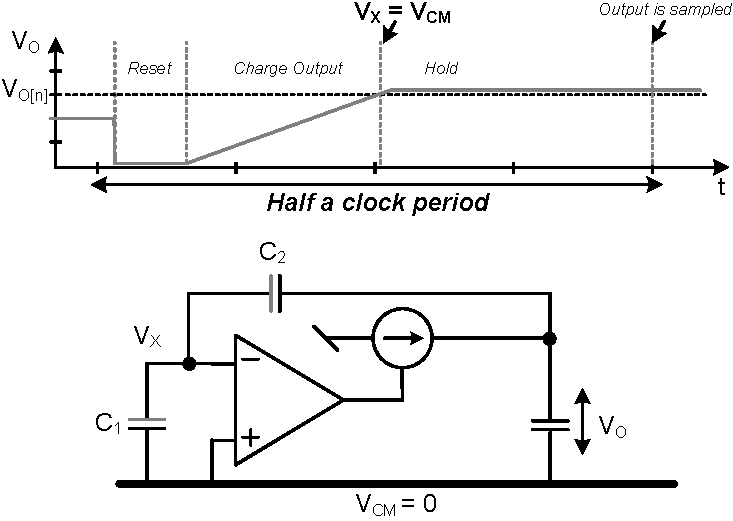
\includegraphics[width=\myfigwidth]{graphics/sc-cbsc}}

   \caption{Opamp based switched-capacitor versus comparator-based switched-capacitor.}
%   \label{cbscfig:opsc_vs_cbsc}
 \end{centering}
\end{figure*}

% \begin{figure}[htbp]
% \centerline{ 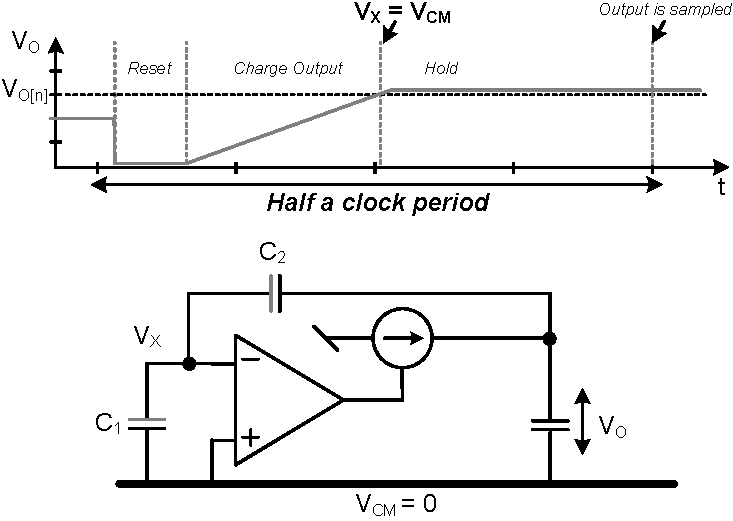
\includegraphics[width=\myfigwidth]{graphics/sc-cbsc}}
%   \caption{Comparator-based switched-capacitor circuit}
%   \label{cbscfig:sc-cbsc}
% \end{figure}


\subsection{Model of MDAC output voltage }
%Modeling is important: equation based
%simulation tools, like MATLAB,  run behavioral level models in
%seconds, compared to minutes for behavioral level models in SPICE and
%days for a full pipelined ADC at transistor level. 

Assume finite resistance in current source. Kirchhoff's current law give the
differential equation
\eqn{
  I_0 = C_o \frac{d V_o(t)}{dt} +  V_o(t)/R_o
}
where $C_o$ is the capacitance at the output, $V_o$ is the
 output voltage, $I_0$ is the current in the current source and
$R_o$ is the output resistance of the current source. Solving the
differential equation yields.
\eqn{
\label{cbsceq:voout}
  V_o(t) = I_0 R_o \left ( 1 - e^{-\dfrac{t}{R_o C_o}} \right)
}
The time $t$ is the sum of $T_{V_I}$ --- the time to charge to the ideal
output voltage ($V_o(t) = 2V_I$)--- and the comparator delay
$T_d$. The ideal charge time $T_{V_I}$ is given by
\eqn{
  T_{V_I} =-ln \left(\frac{-2V_I}{R_o I_0}+1 \right) C_o R_o
} 
To compensate for the comparator delay the comparator threshold
($V_{ct}$) can be changed so
the comparator start switching before $V_o = 2V_I$ is reached. Accordingly,
the charge time can be written as
\eqn{
\label{cbsceq:votime}
  t = -ln\left(-2\frac{V_I-V_{ct}}{R_o I_0}+1\right) C_o R_o + T_d
}
Inserting \req{votime} in \req{voout} results in
\eqn{
\label{cbsceq:vooutfin}
  V_o(t) = 2 e^{-\dfrac{T_d}{R_o C_o}}V_I + I_0R_o[1 - e^{-\dfrac{T_d}{R_0
      C_o}}(1 + 2\dfrac{ V_{ct}}{I_0R_o})]
}
The gain of the amplifier should be two, but from \req{vooutfin} we
see the gain is smaller than two ($2e^{-T_d/R_oC_o}$). This gain error will cause
static non-linearities when a CBSC circuit is used in a pipelined
ADC. The gain error is a function of the comparator delay, the output
resistance and output capacitance. The last term in \req{vooutfin} is the overshoot. 

%Using linear approximation \req{voout} and \req{votime} can be
%simplified. \footnote{The linear approximation of the natural logarithm is $ln(x)
%\approx = x-1$ if $x \approx 1$ and the for the exponential function
%$e^x = x+1$ if $x \approx 0$.}
%Assuming $I_0 R_o >> 1$ \req{votime} is
%\eqn{ 
%\label{cbsceq:votimeas}
%t = \frac{2 V_I C_o}{I_0} - 2\frac{V_{OFF} C_o}{I_0} +
%  T_d
%}
%Assume $t/R_o C_o$ is small, then \req{votimeas}
%inserted in \req{voout} reduce to
%\eqn{
%\label{cbsceq:vooutas}
% V_o  = 2 V_i - 2 V_{ct} + \frac{T_d I_O}{C_o}
%}
%The comparator delay can clearly be cancelled by a threshold change,
%but this assumes the ramp is linear (current source with high output resistance).
%If the capacitance is small, the current large, or the output
%resistance low the output voltage is 
%\req{voout}, and will contain
%infinite harmonics of the input signal.



%-------------------------------------------------------
\section{Implementation}\label{cbsccircuit}
%-------------------------------------------------------
The ADC is an 8-bit differential comparator-based switched
capacitor pipelined ADC. It has continuous time bootstrapped input
switches and comparator-based switched-capacitor MDAC. It differs
from other CBSC ADCs (\cite{brooks07} and \cite{sepke06}) by
being the first fully differential CBSC ADC. A system level diagram is
shown in Fig. \ref{cbscfig:system}. The ADC has seven 1.5-bit pipelined
stages and a 1.5-bit flash-ADC.\footnote{The ADC was
  designed as a 10-bit ADC with eight 1.5-bit stages and a 2 bit flash-ADC. But 
  measurements showed more noise than expected (the noise is dominated
  by the the digital IO). Accordingly, the MDAC in stage 8
  was turned off and the output of the flash-ADC ignored.}

 An on-chip non-overlapping
clock generator generate the clock phases from an external clock. Reference voltages are
generated off-chip. Digital 
error correction is performed off-chip in software for testability. 

Each
pipelined stage is controlled by a 22-bit calibration string,
generated off-chip and written to the ADC through a serial
interface. The calibration string controls the comparator threshold
and current source current. The circuit implementation of blocks is detailed in the 
following sections.
\begin{figure}[htbp]
\centerline{ 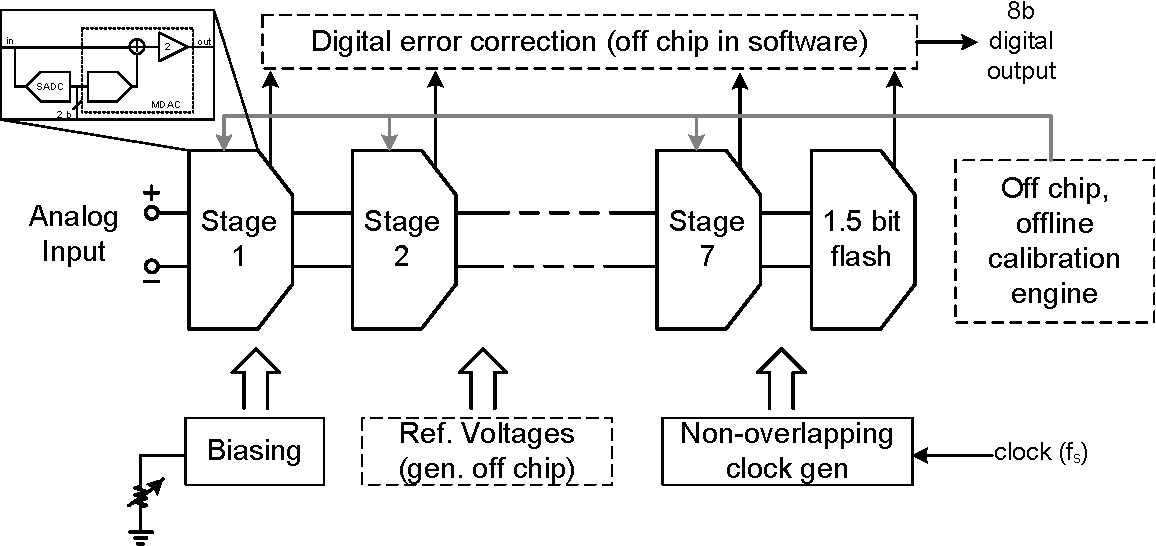
\includegraphics[width=\myfigwidthl]{graphics/scarabtop}}
  \caption{System level diagram of pipelined ADC.}
  \label{cbscfig:system}
\end{figure}


\subsection{Sub ADC}
Each stage in the pipelined ADC has a 1.5-bit analog-to-digital
converter, often referred to as the sub ADC (SADC). The 1.5-bit
architecture use redundancy to correct 
for offset errors in SADC comparators \cite{Lewis92}. As a result,
dynamic comparators can be used, which have large 
offsets but consume little power. In this
converter the resistive divider dynamic comparator is used \cite{cho95}.


\subsection{Stage MDAC architecture}
Fig. \ref{cbscfig:mdac} shows the MDAC of
stage one and the sampling network of stage two.  The stage operates on
four phases $p_1$, $p_2$, $p_r$ and $p_{1a}$. An advanced clock phase
($p_{1a}$) samples the input signal before $p_1$ turns
off, this reduces the problem of signal dependent
charge injection from $p_1$ switches. In phase $p_1$ the comparator is preset
by forcing the comparator inputs to reference voltages $V_{RN}$
and $V_{RP}$, so the output of the comparator is known at the
end of $p_1$. The output is reset in  $p_r$, forcing $V_{XP} <
V_{XN}$.  When $p_r$ goes low the current sources charge the MDAC
output capacitance. The comparator detects when the virtual ground
condition is reached and turn off the current sources. 
The input switches
in the first stage are continuous time bootstrapped switches.

\begin{figure}[htbp]
\centerline{ 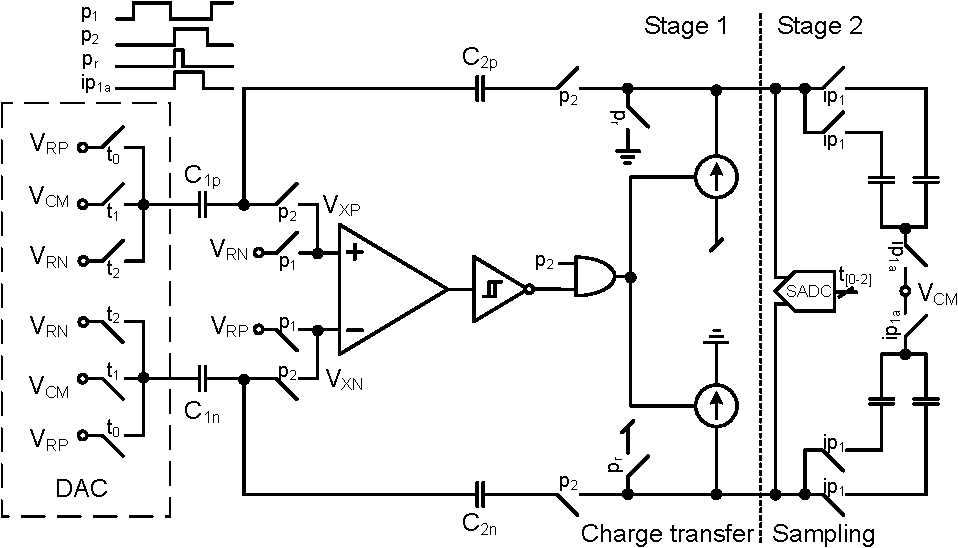
\includegraphics[width=\myfigwidthl]{graphics/mdac}}
  \caption{Stage one during charge transfer and stage two during sampling.}
  \label{cbscfig:mdac}
\end{figure}

\subsection{Continuous time bootstrapped switch}
Bootstrapped switches are used to reduce the signal dependent charge
injection and signal dependent 
switch conductance \cite{abo99}. In bootstrapped switches a constant
gate-source voltage is applied to the switch. One method  charges a
capacitor to a fixed voltage when switch is 
off, and when the switch is turned on the capacitor is connected
between the gate and source of the switch, thus acting as a battery to keep the gate-source voltage constant \cite{abo99}. 

Another approach is continuous time bootstrapping
\cite{jakonis02}. A source follower tracks the
input signal, the gate-source voltage of the switch is set by
the gate-source voltage of the source follower. Fig. \ref{cbscfig:ctbs}
shows the continuous time bootstrapped switch. Thick
oxide transistors (marked in Fig. \ref{cbscfig:ctbs} by 
thick gates) are used to reduce reliability concerns.

The source follower $M_2$ is biased by $M_1$. An inverter ($M_3$ and
$M_4$) control the gate voltage of the switch ($M_S$), the inverter switches
between the level shifted input ($V_A$) and ground. When the switch is
on ($p_1$ high) $M_5$ shorts the bulk of $M_S$ to the input, reducing the body
effect and improving reliability (keeps gate bulk constant). When the
switch is off $M_6$ shorts the bulk to ground to avoid forward biasing
the bulk-drain PN junction.
\begin{figure}[htbp]
\centerline{ 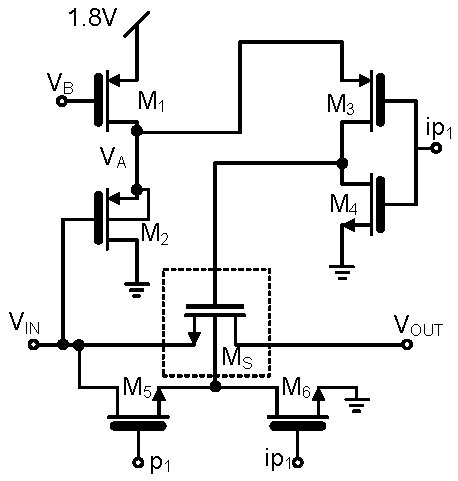
\includegraphics[width=\myfigwidthb]{graphics/ctbs}}
  \caption{Continuous time bootstrapped switch.}
  \label{cbscfig:ctbs}
\end{figure}

% It is on when $p_1$ is high and off when $p_1$ is low, $ip_1$
% is $p_1$ inverted. The source follower ($M_2$) is biased by $M_1$, and the source
% of $M_2$ tracks the input voltage, but shifted by the gate-source
% voltage of $M_2$. The voltage $V_{A} - V_{IN}$  is constant if the
% source follower has a gain of one. The gate voltage of switch $M_2$
% is controlled by inverter $M_3$ and $M_4$, which switches between the
% level shifted input voltage at $V_A$ and ground. In 
% \cite{jakonis02} the output of the source follower ($V_A$) was connected
% to gate of $M_2$ and the switch was turned off by
% forcing $V_A$ to ground. If $M_3$ in Fig. \ref{cbscfig:ctbs} is replaced
% with a short an equivalent schematic is produced. There
% are two problems with shorting $V_A$ to ground. When the switch turns on
% $dV_A/dt$ will be large and will kick-back through $C_{GS,M_2}$ to the input
% voltage $V_{IN}$. The effects of the kick-back must settle before
% the input voltage is sampled. With $M_3$ $V_A$ is not connected to the gate of
% $M_S$  when it is turned off, which reduces kick-back through
% $M_2$. Also, with $M_3$ power dissipation for high speed operation is reduced. Assume $V_X$
% is forced to ground, when $M_S$ turns on $M_2$ is in the linear
% region, and to reach reach active region $V_A$ has to be larger
% than the effective overdrive. The capacitance in node $V_A$
% is dominated the gate-source capacitance of $M_2$ and the capacitance of the
% reversed biased PN junction between the PMOS N-Well and
% substrate. This capacitance has to be charged through $M_1$, if
% fast turn on times are required a larger bias current is
% required since the slewrate is $SR_{V_A} = I_{M_1}/C_A$. With $M_3$
% $V_A$ continuously track the input voltage and 
% $M_2$ is always in active region, accordingly the bias current
% $I_{M_1}$ can be smaller.
 
%Switches $M_5$ and $M_6$ serve
%multiple purposes, they linearize
%the switch when on through keeping $V_{BS} \approx 0$,  $M_5$ improves
%reliability by ensuring
%that the gate bulk voltage of $M_S$ does not exceed maximum ratings, and
%%$M_6$ ensures that the bulk-drain PN junction is not forward biased when the
%switch is off. 


\subsection{Comparator with adjustable threshold}
A two-stage continuous time amplifier
(Fig. \ref{cbscfig:comp}) with a differential first stage and single
ended common source second stage is used as the comparator. 

\begin{figure}[htbp]
\centerline{ 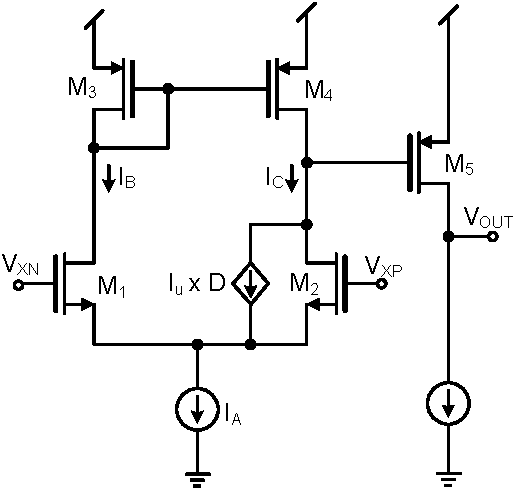
\includegraphics[width=\myfigwidthb]{graphics/comp}}
  \caption{Comparator with adjustable threshold.}
  \label{cbscfig:comp}
\end{figure}

In phase $p_1$ the comparator inputs
are reset to $V_{RN}$ and $V_{RP}$ (as shown in
Fig. \ref{cbscfig:mdac}), so the output is known at the end of $p_1$.
With this
preset the design of control logic between comparator and current sources
is simplified. Phase $p_2$ start by resetting the MDAC outputs,
this cause $V_{XN}$ to increase and $V_{XP}$ to decrease. When reset
is complete the current sources start charging the MDAC outputs, as a result
$V_{XN}$ falls and $V_{XP}$ rise. 

Fig. \ref{cbscfig:comp_p}, Fig. \ref{cbscfig:comp_z}, and
Fig. \ref{cbscfig:comp_n} 
%Fig. \ref{cbscfig:comp_th} 
shows
$V_{XN}$ and $V_{XP}$ as a function of time for different comparator
thresholds ($V_{ct}$). 
 The comparator should turn off current
sources when $V_{XP} = V_{XN}$, but because the
comparator has a delay
($T_d$) the current sources  turn off later, causing an overshoot  (Fig. \ref{cbscfig:comp_p}).
Adjusting the threshold of the 
comparator  changes the amount of overshoot. If $V_{ct}$
is adjusted optimally there is no overshoot  (Fig. \ref{cbscfig:comp_z}).
If $V_{ct}$ is lower than the optimal value the 
output undershoots (Fig. \ref{cbscfig:comp_n}). From the figure we see
that a non-optimal threshold cause an offset in the MDAC output, as
shown in \req{vooutfin}. If the offset is small it is corrected by the
digital error correction inherent to 1.5-bit stage architecture. Although, the
extra offset from the overshoot increase the demands on the dynamic
comparators because the sum of offsets must be less than $\pm
V_{REF}/4$ in a 1.5-bit stage.

The comparator threshold is controlled with a 6-bit current DAC in
parallel with $M_2$, shown as a controlled current source. In Fig. \ref{cbscfig:comp} $I_u$ is a unit current
and $D$ is an integer given by $D = 2^0b_0 + 2^1b_1 + 2^2b_2 + 2^3b_3
+2^4b_4 + 2^5b_5$.  The current in the current source $I_A$ is the sum of the
two branch currents ($I_A = I_B + I_C$). The comparator threshold is
defined as the differential input voltage when the branch currents are
equal ($I_B = I_C$). Equal currents occur when
\eqn{
  \beta V_{EFF,1}^2 = \beta V_{EFF,2}^2 + I_u \times D 
}
where $\beta = \frac{1}{2}\mu_n C_{ox} \frac{W}{L}$ and $V_{EFF,X}$ is
the effective gate overdrive of transistors $M_X$. If $D=0$ the
currents are equal when the effective gate overdrives are equal,
which occurs when the positive and negative inputs are equal. If $ D >
0$ the currents are equal when the effective 
overdrive of $M_1$ is larger than the effective overdrive of $M_2$,
which occurs when $V_{IN} > V_{IP}$. 
%We know the delay is too long --- the delay is positive, and we would
%like it to be zero --- so there is no point in increasing the
%delay with a similar controlled current source in parrallel with
%$M_1$. 

The nominal
delay of the comparator (including Schmitt trigger and logic gates) is
$T_d = 0.5ns$. With the 6-bit DAC the effective delay of the comparator
can be controlled from $T_d = -0.9ns$ to $T_d = 0.5ns$.
%\begin{minipage}


\begin{figure*}[htbp]
 \begin{centering}
 \subfigure[Comparator threshold equal to zero]{\label{cbscfig:comp_p} 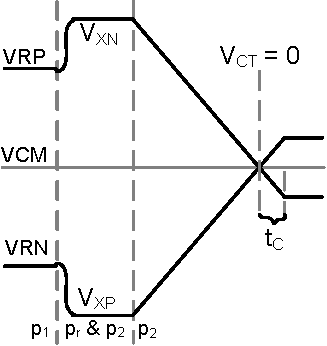
\includegraphics[width=\myfigwidthc]{graphics/comp_p}}
 \subfigure[Optimal comparator threshold]{\label{cbscfig:comp_z}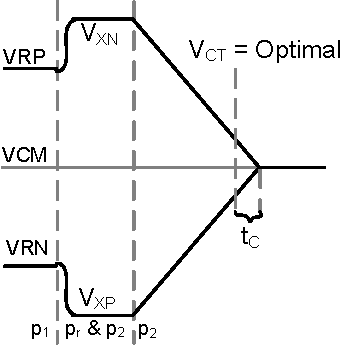
\includegraphics[width=\myfigwidthc]{graphics/comp_z}}
 \subfigure[Comparator threshold less than the optimal value]{\label{cbscfig:comp_n} 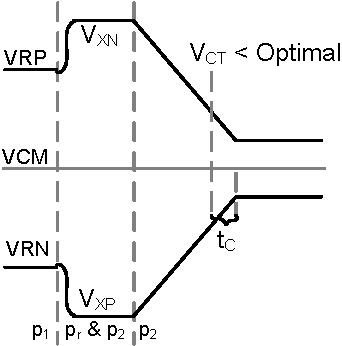
\includegraphics[width=\myfigwidthc]{graphics/comp_n}}
   \caption{Voltage versus time for the nodes $V_{XN}$ and $V_{XP}$ as
  a function of comparator threshold.}
%   \label{cbscfig:comp_th}
 \end{centering}
\end{figure*}



% \begin{figure}[htbp]
%   \centerline{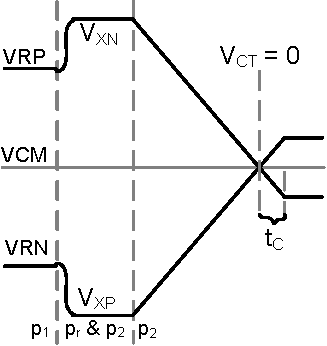
\includegraphics[width=\myfigwidthb]{graphics/comp_p}}
%   \caption{Comparator threshold equal to zero}
%   \label{cbscfig:comp_p}
% \end{figure}

% \begin{figure}[htbp]
%   \centerline{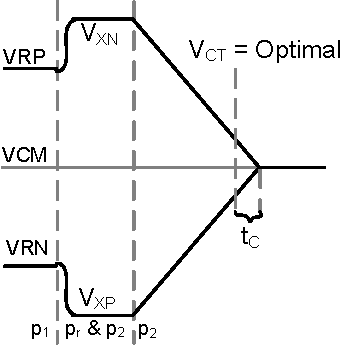
\includegraphics[width=\myfigwidthb]{graphics/comp_z}}
%   \caption{Optimal comparator threshold}
%   \label{cbscfig:comp_z}
% \end{figure}

% \begin{figure}[htbp]
%   \centerline{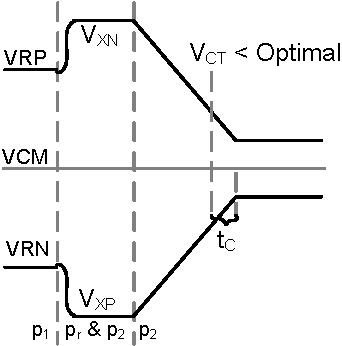
\includegraphics[width=\myfigwidthb]{graphics/comp_n}}
%   \caption{Comparator threshold less than the optimal value}
%   \label{cbscfig:comp_n}
% \end{figure}


\subsection{Current sources}
We used regulated cascode current sources to achieve high output
resistance
(Fig. \ref{cbscfig:current}). A PMOS current source is used for the pull
up current, and a NMOS current source is used for the pull down
current. Both the cascode and the common source transistors are turned
off when the current source is turned off.

 A single boost amplifier is
shared between current sources to save power (as shown in \reg{current}). The amplifier sees a variable
capacitive load (the load varies with how many current sources are
enabled), which affects settling and stability, both manageable
challenges.

 The 
current source is programmed with an 8-bit word, with
6-bit resolution due to intentional overlap. The NMOS and
PMOS sources are controlled separately. If the PMOS and NMOS currents
are different the output common mode of the MDAC will be different
from $(VDD-VSS)/2$. Simulations suggest that common
mode feedback circuit is unnecessary. 

\begin{figure}[htbp]
\centerline{ 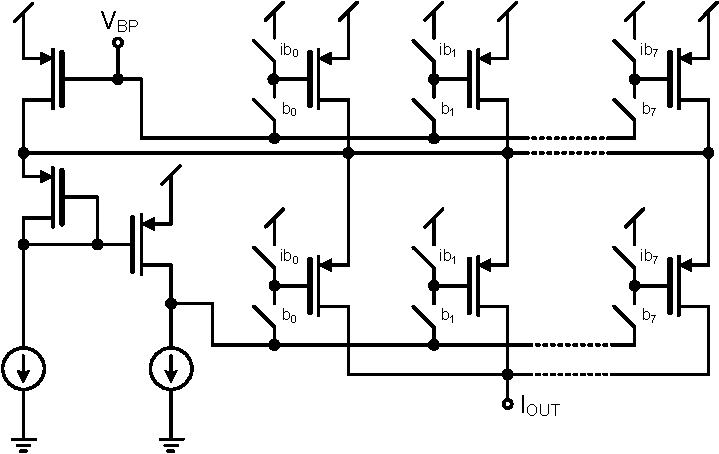
\includegraphics[width=\myfigwidth]{graphics/current}}
  \caption{Programmable regulated cascode current source with high output resistance.}
  \label{cbscfig:current}
\end{figure}

\subsection{Bias circuits, digital error correction and reference voltages}
The pipelined core has a simple bias circuit with two external bias
currents. One bias current is copied to all analog blocks 
and the other bias current control the delay of current starved inverters used to
generate the reset phase ($p_r$). Current mirrors are cascoded when possible. External reference voltages are used for
testability, so the power
consumed by the references is not included in reported
power dissipation. The digital outputs from the SADCs are brought
off-chip by CMOS logic IO buffers. Synchronization,
recombination and digital error correction of the output bits is performed in software.

%-------------------------------------------------------
\section{Calibration}\label{cbsccalibration}
%-------------------------------------------------------
In CBSC some form of auto-zeroing or calibration is required. This can
be seen from \req{vooutfin}, the overshoot is proportional to
$I_0$ and inversely proportional to the output capacitance of the
MDAC. Both current and capacitance change with process corner. 

Each stage has three calibration words, one for each
current source and one for the comparator. The calibration
word for the current sources is 8-bit, and 6-bit for the comparator threshold,
in total, 22-bits per stage. All seven stages are calibrated, which
results in $2^{154}-1$ combinations, a  large
solution space.

 It is impossible to test all combinations in such a large solution
space.\footnote{Assuming one combination could be tested each clock
  cycle it would take $48\times 10^{30}$ years to test all
  combinations} So we 
use two different calibration  
algorithms: one deterministic time comparator threshold calibration, and a
non-deterministic time genetic algorithm. The
first algorithm calibrate the  comparator delay to correct for the overshoot, while the
second algorithm also calibrate the current in the current sources.

\subsection{Deterministic time comparator threshold calibration }
A flowchart of the calibration algorithm is shown in Fig.
\ref{cbscfig:cal_off}.  The current source word $W_{I[N]}$ is
the same for all stages, so all stages will have the
same nominal current. Initially all currents are set to zero,
$W_{I[0-7]} = 0 $. The comparator threshold word $W_{C[N]}$ is also set to
zero for all stages ($W_{C[N]} = 0$). The maximum value of the comparator
threshold is $W_{CMAX} = 2^6-1$, and the minimum value is $W_{MIN} =
0$. $M$ and $N$ are the indexes of the inner and outer loop.

Calibration starts by turning on the current in the first stage ($W_{I[0]}
= W_{IDEF}$, where $W_{IDEF}$ is a sufficient current for the speed of
the ADC). The comparator threshold is set to half the
distance between the maximum and minimum word given by
\eqn{
W_{C[N]} = \left\lceil
  \dfrac{W_{CMAX} + W_{CMIN}}{2}\right\rceil
}
The ADC is updated with the new calibration words --- in the prototype the
calibration algorithm is written in software and the calibration
words are written to the ADC using a serial interface, however, the
calibration algorithm can easily be integrated in hardware. 

The mean value of the
output is calculated using a window length of $L$. The  run
time is proportional to window length, and the window length set the
accuracy of the mean. We assume the input signal is a zero mean sinusoid
close to Nyquist, so a window length of $L=2^B$ is sufficient. The
sign of the calculated mean plus a 
reference offset $x_{REF}$ is evaluated. If it is positive the
comparator threshold is increased ($W_{CMIN} =
W_{C[N]}$). If it is negative the comparator threshold is
reduced ($W_{CMAX} =
W_{C[N]}$). The inner loop index is updated ($M = M +1$), and the search
continues. The inner loop performs a binary search for the correct
comparator threshold in each stage. The outer loop turns on
more and more stages as the inner loop completes. 

If we assume the
time spent writing 
the calibration words to the ADC is insignificant the calibration algorithm will
complete after  $7 \times 7 \times 256 = 12.5k$ clock
cycles. A genetic algorithm was used to verify that this calibration
algorithm finds a solution close to optimum. 
\begin{figure}[htbp]
\centerline{ 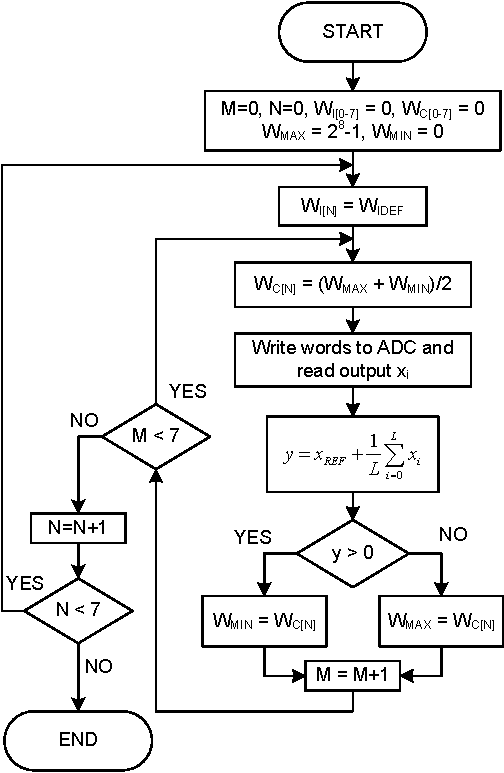
\includegraphics[width=\myfigwidthb]{graphics/cal_off}}
  \caption{Deterministic time comparator threshold calibration.}
  \label{cbscfig:cal_off}
\end{figure}

\subsection{Non-deterministic calibration}
To verify the comparator threshold calibration a genetic algorithm is used.
A genetic algorithm
models evolution and has been shown to find solutions for
large search spaces \cite{back97}. The disadvantage of the genetic algorithm is the
non-deterministic run time, since it cannot be determined analytically
how long it takes before a good solution is found. The genetic
algorithm varies both current and comparator
threshold in the ADC. 


%-------------------------------------------------------
\section{Experimental results}\label{cbscresults}
%-------------------------------------------------------

\subsection{Results of calibration}
The input signal during calibration is a sinusoidal input close to
the Nyquist frequency  ($f_i = 29.4MHz$).
%Fig. \ref{cbscfig:inl_cal}
%\myinlref
\reg{inl_nocal}, \reg{inl_offcal} and \reg{inl_gacal}
 shows the measured \textit{integral non-linearity} (INL) and
\textit{differential non-linearity} (DNL) for three different cases. Fig.
\ref{cbscfig:inl_nocal} shows the INL and DNL for the default calibration
words set before production based on simulation. Here the
comparator threshold is too low, which results in an overshoot. For the un-calibrated
case the ENOB is 2.4-bits. 

Using deterministic time comparator
threshold calibration the INL and DNL
improves from +36/-9 LSB to +1.6/-1.8 LSB, as shown in Fig. \ref{cbscfig:inl_offcal}. With comparator
threshold calibration 
the ENOB is 6.5-bit. The INL shows signs of a gain error, and
multiplying the bits from the first stage by 1.022 improve the ENOB to
6.9-bit. From \req{vooutfin} this suggest that either the comparator
delay is too long, the output resistance is to  low or capacitance
is to low.

 Using the genetic 
algorithm a better solution is found, shown in
Fig. \ref{cbscfig:inl_gacal}. The best solution improve the ENOB by
0.5-bit, resulting in a peak ENOB of 7.05-bit. This solution use less
current in the first stage than used with comparator threshold
calibration, which does increase the output resistance of 
the current sources in the first stage. According to \req{vooutfin} this would
reduce the gain error, but reduced
output resistance has not been confirmed as the cause of the gain
error.

The best solution is
used for the remainder of the measurements. 

%\myinl
% \begin{figure}[htbp]
% \centerline{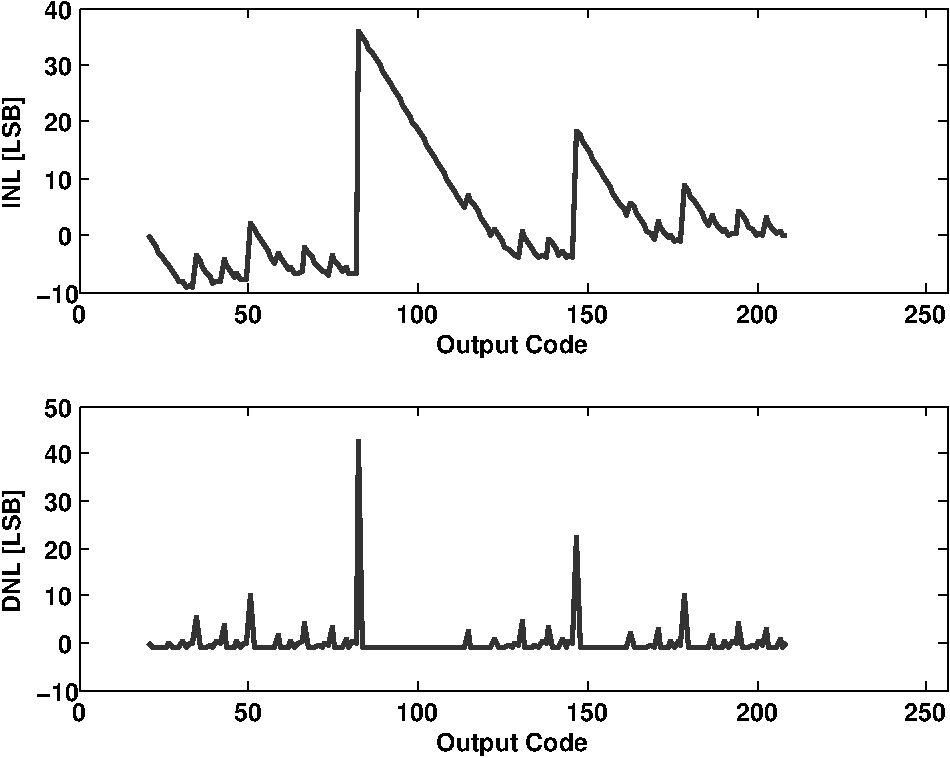
\includegraphics[width=\myfigwidth]{graphics/inl_nocal}}
%  \caption{No calibration, default values set before before
%    production}
% \label{cbscfig:inl_nocal} 
% \label{cbscfig:inl_cal}
% \end{figure} 

% \begin{figure}[htbp]
% \centerline{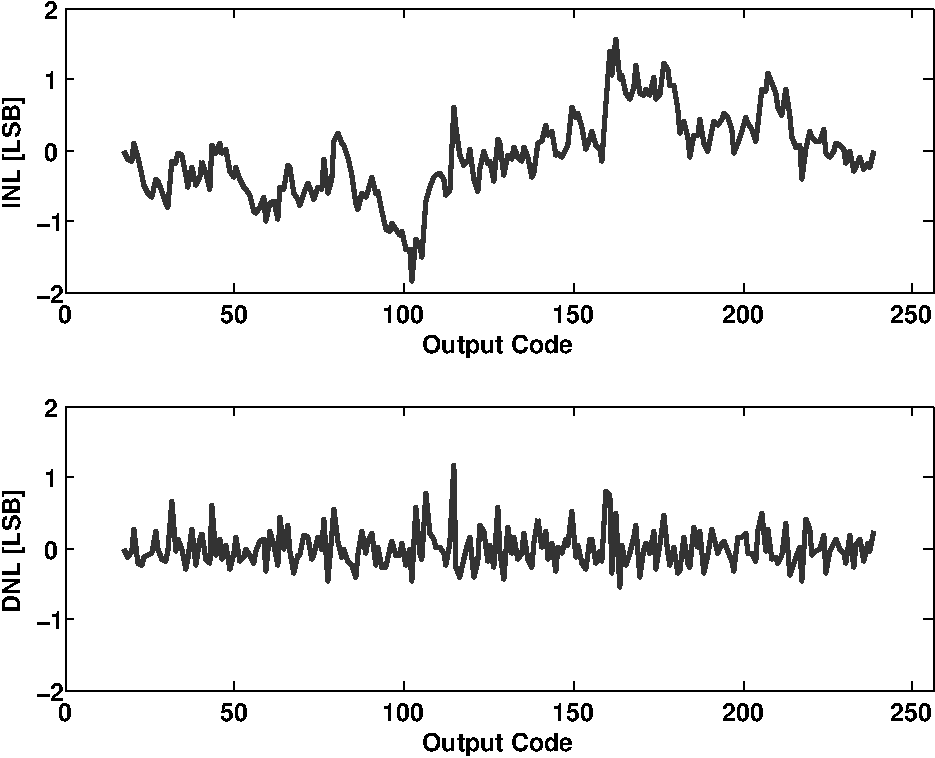
\includegraphics[width=\myfigwidth]{graphics/inl_offcal}}
% \caption{Deterministic calibration of comparator
%  thresholds with current fixed}
% \label{cbscfig:inl_offcal}
% \end{figure}

% \begin{figure}[htbp]
% \centerline{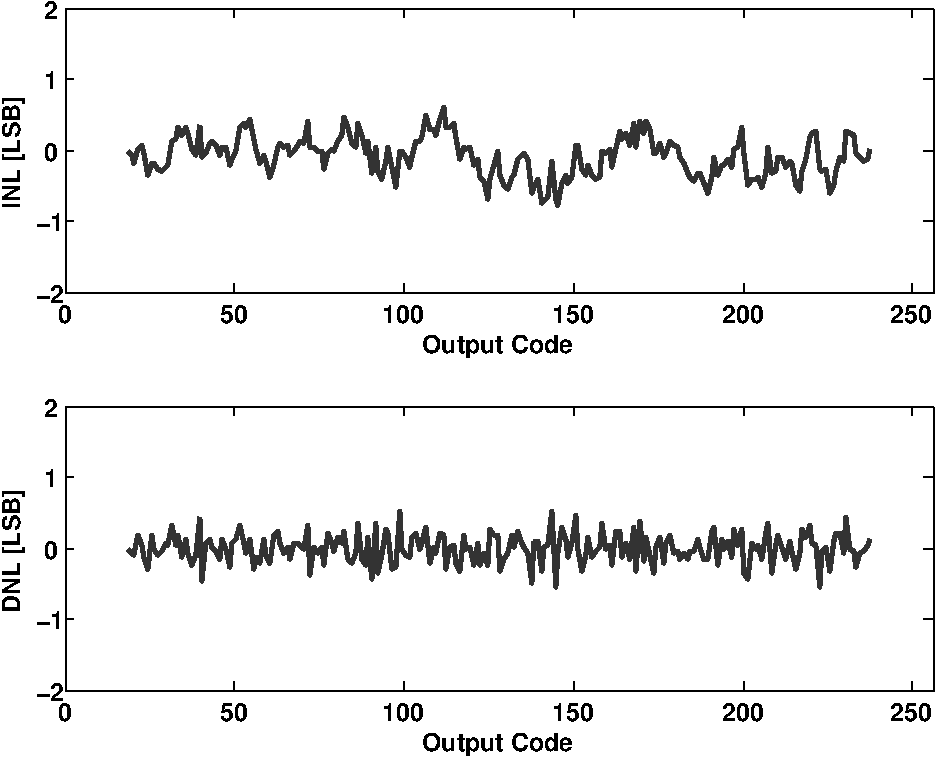
\includegraphics[width=\myfigwidth]{graphics/inl_optcal}}
%  \caption{Non-deterministic calibration of positive and negative current plus
%  comparator threshold using a genetic
%  algorithm.}
% \label{cbscfig:inl_gacal}
% \end{figure}


\begin{figure*}[htbp]
 \begin{centering}
 \subfigure[No calibration, default values set before before production.]{\label{cbscfig:inl_nocal} 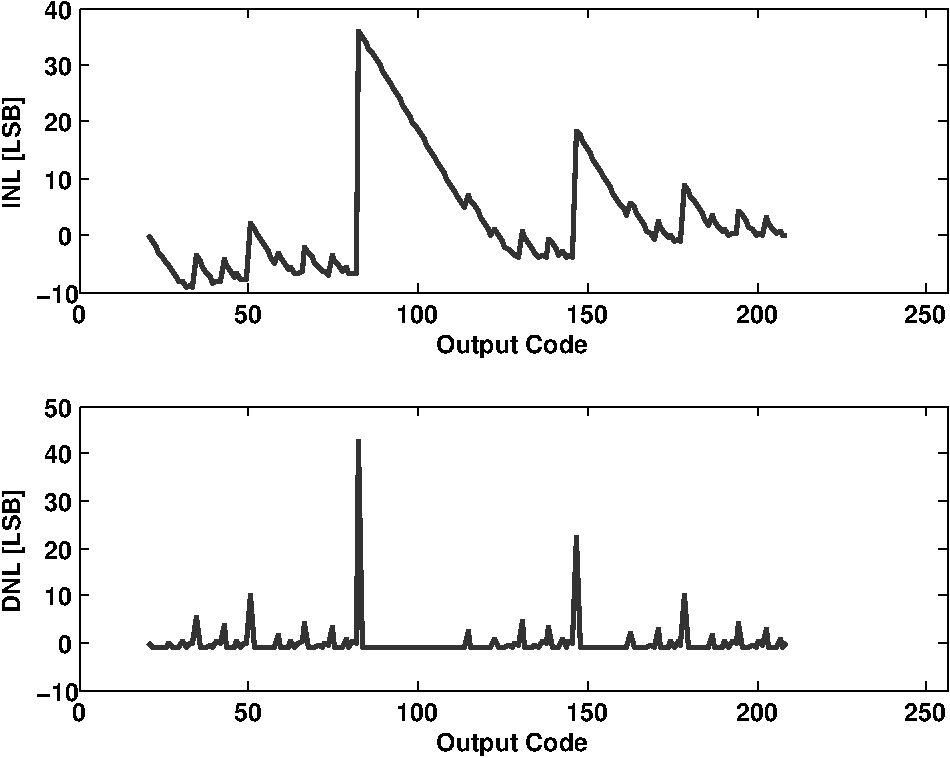
\includegraphics[width=\myfigwidthe]{graphics/inl_nocal}}
 \subfigure[Deterministic calibration of comparator
 thresholds with current fixed.]{\label{cbscfig:inl_offcal}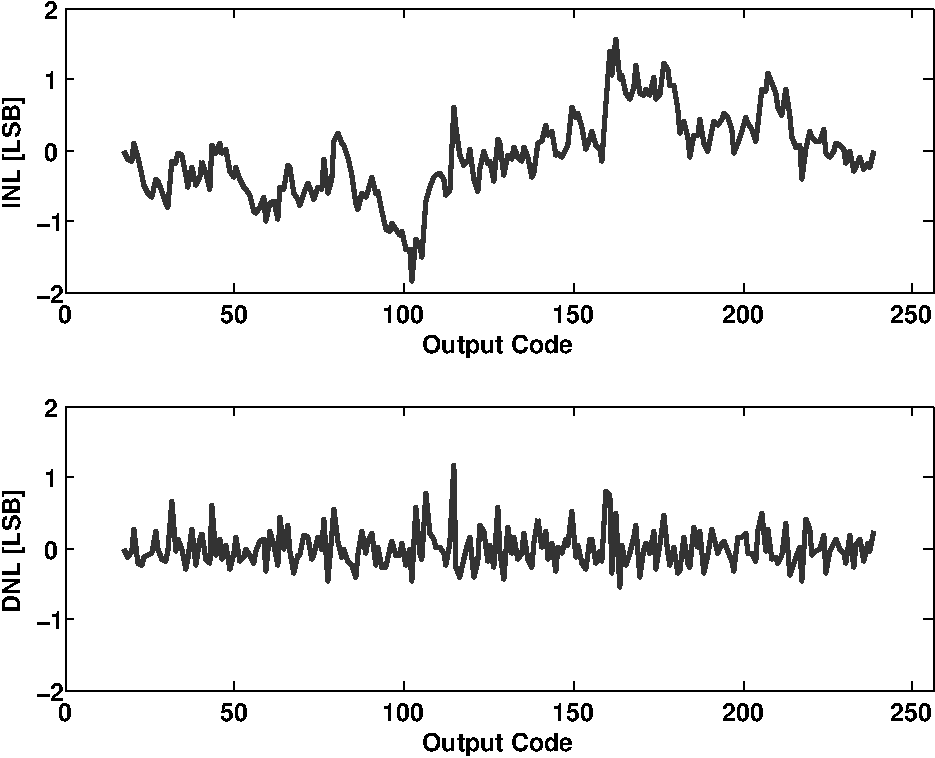
\includegraphics[width=\myfigwidthe]{graphics/inl_offcal}}
 \subfigure[Non-deterministic calibration of positive and negative
 current, and
 comparator threshold using a genetic algorithm.]{\label{cbscfig:inl_gacal} 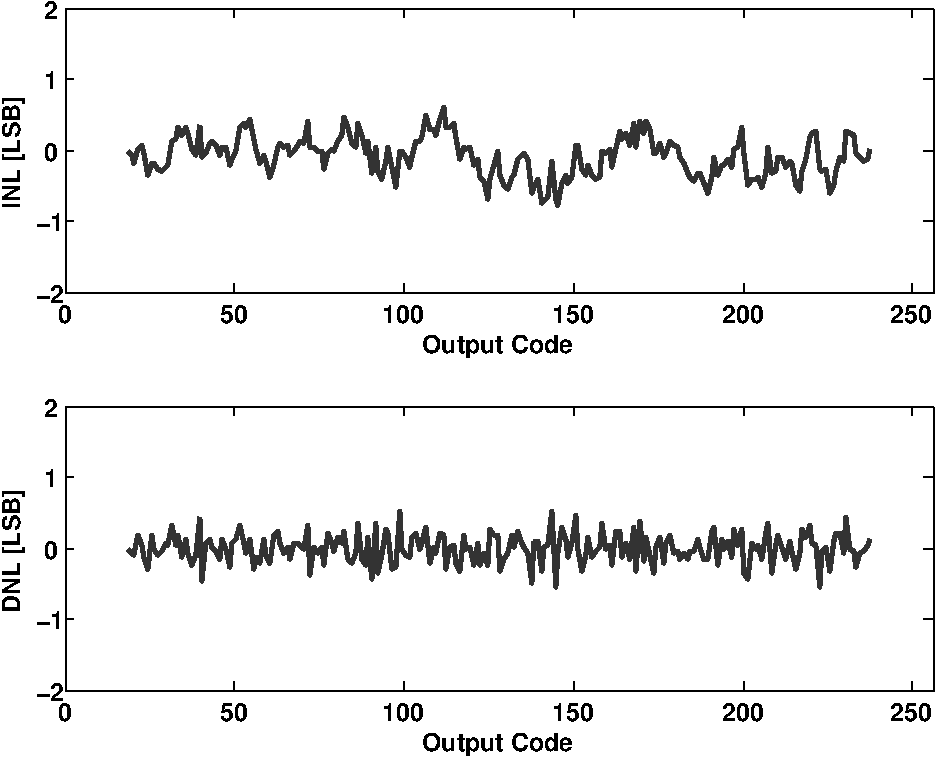
\includegraphics[width=\myfigwidthe]{graphics/inl_optcal}}
   \caption{INL and DNL for uncalibrated, offset calibration and
     genetic algorithm }
%   \label{cbscfig:inl_cal}
 \end{centering}
\end{figure*}

\subsection{Measured power and accuracy}
%Measurment results and the chip micrograph is shown in Fig \ref{cbscfig:meas_res}.
%The micrograph of the ADC is shown in Fig. \ref{cbscfig:mc}.
A summary
of the ADC performance is shown in Table 
\ref{cbsctab:summary}. It achieves a \textit{signal-to-noise and distortion ratio} (SNDR)
of 44.2-dB (7.05-bit) at Nyquist, with a sampling frequency of
60MS/s and a power dissipation of 8.5mW (5.9mW for ADC core, 2.3mW
for clock generation and distribution, and 0.3mW for input switches), which result in a Walden figure of
merit of 1.07 pJ/step\footnote{ $FOM = P/2^B f_s$} and a Thermal
figure of merit of 8.09fJ/step.\footnote{$FOM = P/2^{2B}f_s$} An input
signal amplitude of -1 dBFS is used. The micrograph of the ADC is shown in Fig. \ref{cbscfig:mc}.

The ADC has a
\textit{spurious free dynamic range} (SFDR)  of 60-dB close to Nyquist. The SNDR and SNR change little with input
frequency, and the effective resolution bandwidth extend well beyond
the Nyquist frequency (Fig \ref{cbscfig:sndrvsfreq}). The SFDR change
with frequency and is maximum close to Nyquist. The calibration
algorithm used this frequency and we assume that is why the SFDR
best at that frequency. 

A 8192 point FFT of the ADC output is shown in Fig \ref{cbscfig:hfft}. Coherent sampling and a Hanning
window is used to avoid spectral leakage of the fundamental. 



Simulation of the ADC showed a peak SNDR of 9-bits (the ADC was designed
as a 10-bit ADC), but as
\cite{brooks07a}, we measured more noise than expected. Most of the
extra noise appear to be coming from digital IO. As \cite{brooks07a} we noted a strong
correlation between digital IO supply voltage and noise level in the
ADC. In theory the power supply rejection is better in a differential
design, which could suggest that there is mismatch between the differential
paths in the ADC, but this has not been quantified. As a result of the
noise from digital IO, the IO used a voltage supply of 0.84V, which limited
the speed of the converter to 60MS/s. Increased speed can be
achieved, but only by increasing the digital IO supply voltage, which in turn
increase the noise (5.5-bit ENOB at 1.2V digital IO supply voltage).

%We believe the harmonic
%content in Fig. \ref{cbscfig:hfft} come from a combination of mismatch
%between current sources . From \req{voout} we can clearly see that with
%high currents, low capacitance and finite current source resistance the exponential
%in the output voltage create harmonics of the fundamental. A MATLAB
%model using \req{voout} replicate the FFT of Fig. \ref{cbscfig:hfft} with
%similar harmonic content and SNDR. The MATLAB model use the same
%capacitor scaling used in the ADC, equivalent currents and equivalent
%current source output resistance, and a mismatch of $ 2 \mu A$  between PMOS and NMOS
%current sources. 

% \begin{figure}[htbp]
% \centerline{ 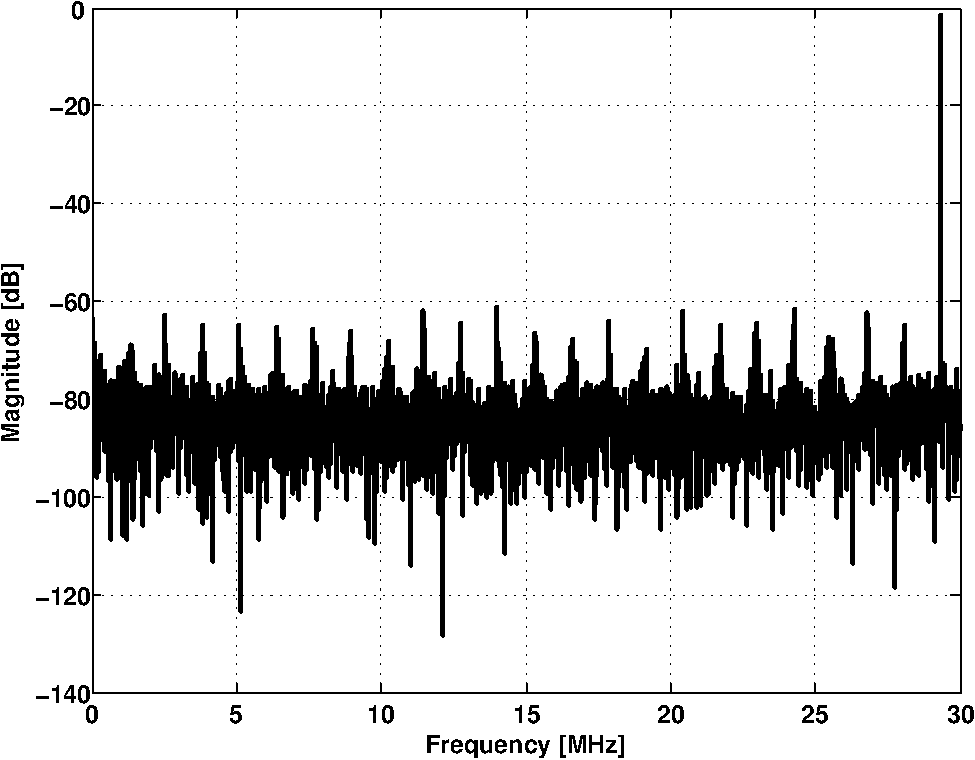
\includegraphics[width=\myfigwidth]{graphics/hf_fft}}
%   \caption{A 8192 point FFT of the ADC output }
%   \label{cbscfig:hfft}
% \end{figure}

\begin{figure*}[htbp]
 \begin{centering}
 \subfigure[A 8192 point FFT of the ADC
 output.]{ \label{cbscfig:hfft} 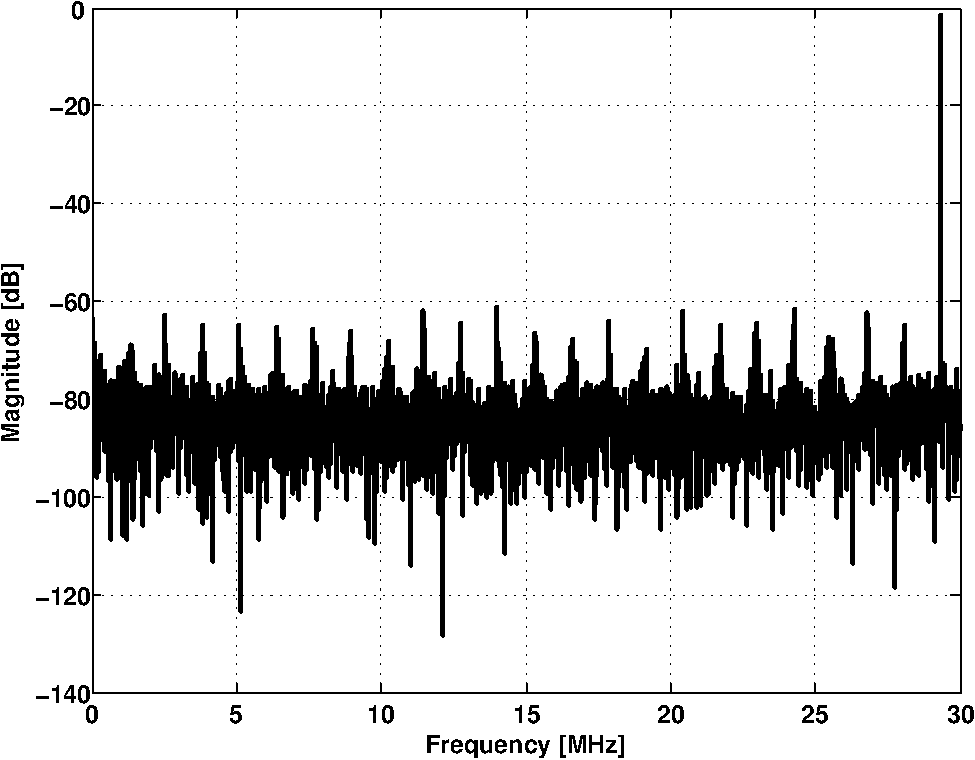
\includegraphics[width=\myfigwidthe]{graphics/hf_fft} }
 \subfigure[SNDR, SNR and SFDR versus frequency, sampling frequency is
 60MS/s. Calibration words are constant. ]{\label{cbscfig:sndrvsfreq} 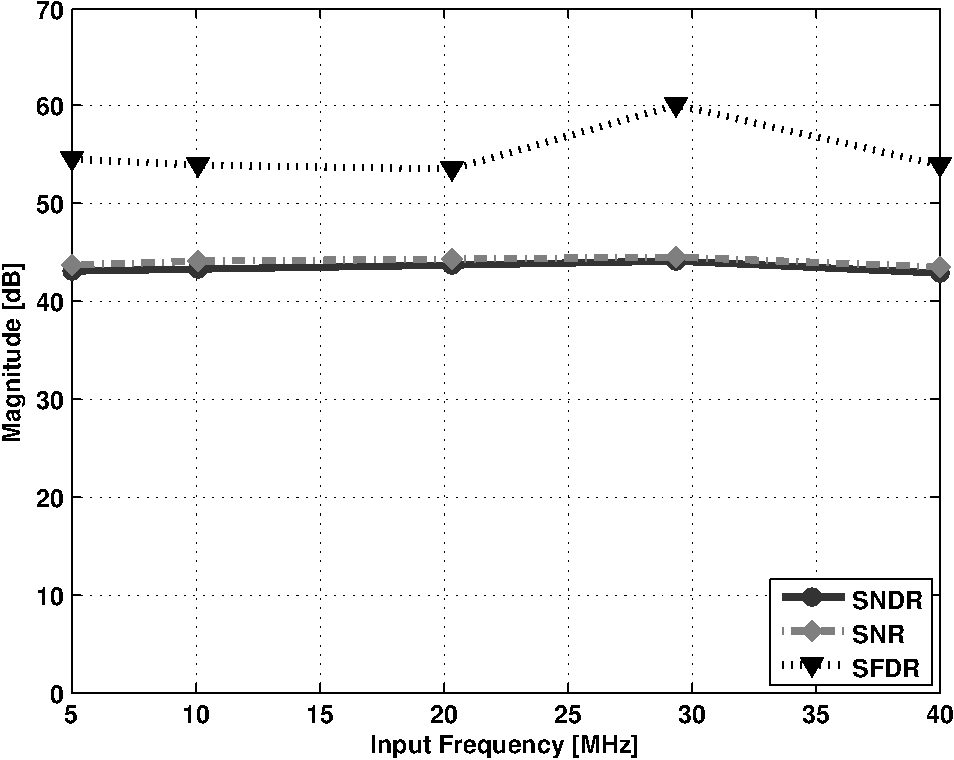
\includegraphics[width=\myfigwidthe]{graphics/sndrvsfreq}}
 \subfigure[Chip micrograph. Stage 8 and flash-ADC are not used.]{ \label{cbscfig:mc} 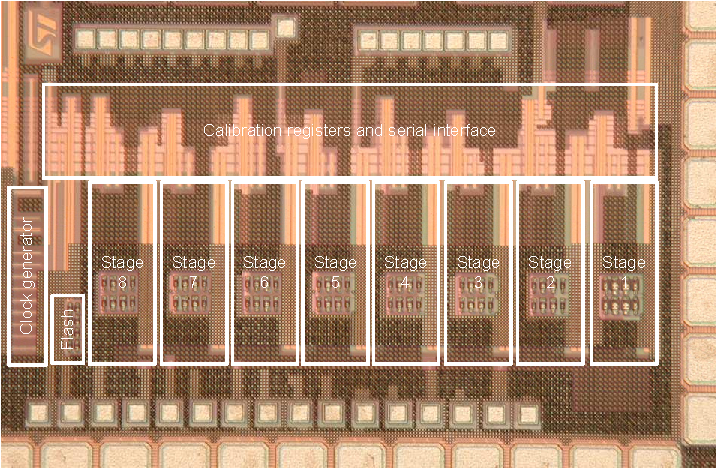
\includegraphics[width=\myfigwidthe]{graphics/mc}}
   \caption{FFT of ADC output, dynamic parameters versus frequency,
     and chip micrograph.}
 \end{centering}
\end{figure*}


% \begin{figure}[htbp]
% \centerline{ 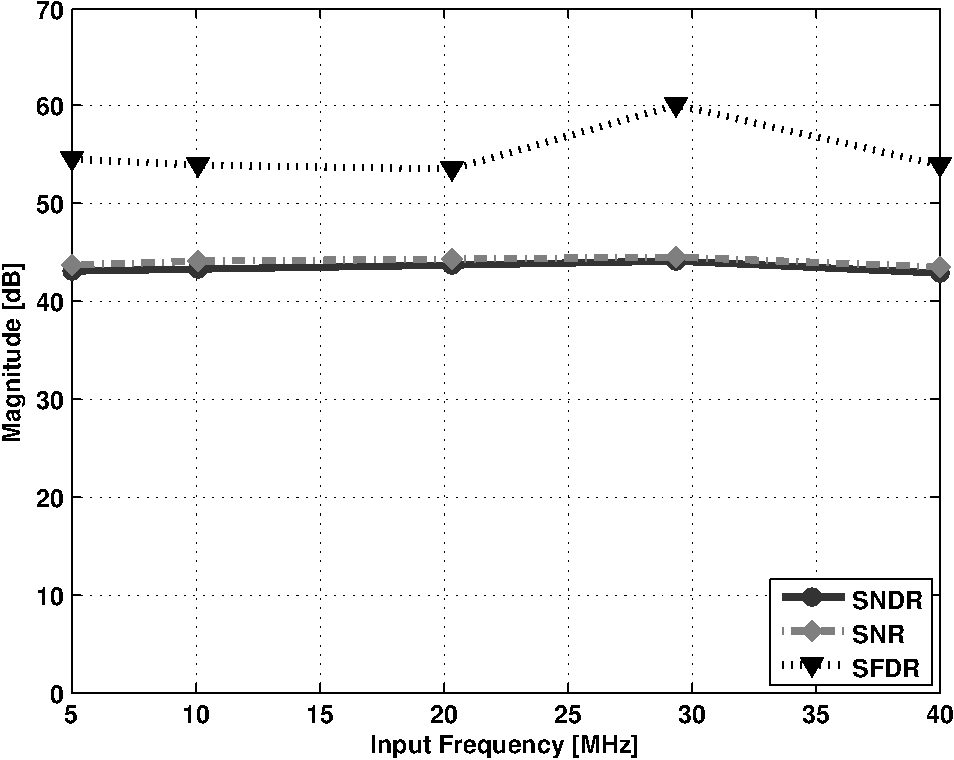
\includegraphics[width=\myfigwidth]{graphics/sndrvsfreq}}
%   \caption{SNDR, SNR and SFDR versus frequency, sampling frequency is
%     60MS/s. Calibration words are constant.}
%   \label{cbscfig:sndrvsfreq}
% \end{figure}



% \begin{figure}[htbp]
% \centerline{ 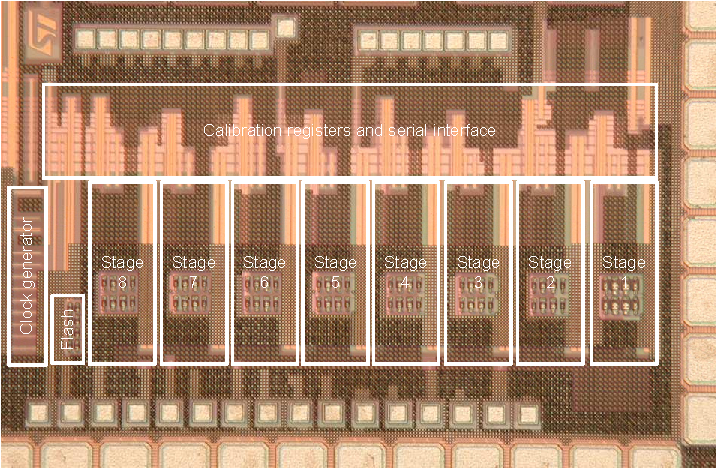
\includegraphics[width=\myfigwidth]{graphics/mc}}
%   \caption{Chip micrograph. Stage 8 and flash-ADC are not used.}
%   \label{cbscfig:mc}
% \end{figure}




\begin{table}[htbp]
\centering
\renewcommand{\arraystretch}{1.3}
\caption{ Summary of calibrated ADC performance  }
\label{cbsctab:summary}
\begin{tabular}{l|r}
Technology & 1.2V/1.8V 90nm CMOS\\
\hline
Sampling Frequency & 60 MS/s\\
\hline
Resolution & 8 bits \\
\hline
Full scale input & 0.8V \\
\hline
Size & 0.85mm x0.35 mm\\
\hline
DNL (LSB)& 0.52 / -0.54\\
\hline
INL (LSB)& 0.6 / -0.77\\
\hline
SNR (29.4MHz input) & 44.5 dB\\
\hline
SNDR (29.4MHz input) & 44.2 dB\\
\hline
SFDR (29.4MHz input) & 60 dB\\
\hline
ADC core power & 5.9mW\\
\hline
Clock power & 2.3mW\\
\hline
Input switches (1.8V) & 0.3mW\\
\hline
Waldon Figure of Merit & 1.07 pJ/step\\
\hline
Thermal Figure of Merit & 8.09 fJ/step\\
\hline
\end{tabular} 
\end{table}




%-------------------------------------------------------
\section{Conclusion}
%-------------------------------------------------------
The first differential comparator-based switch
capacitor (CBSC) pipelined ADC was presented. The switched-capacitor multiplying
digital-to-analog converter (MDAC)
use current sources and a comparator to do charge transfer. Continuous
time bootstrapped switches were used in the first stage to reduce signal dependent switch
resistance. A simple calibration algorithm correct for
comparator delay variation due to manufacturing. Calibration reduce
ramp overshoot, which dominate the non-linearity in CBSC ADCs. The ADC was produced in a 90nm
low-power CMOS technology. The ADC core is 0.85mm x 0.35mm, with a
1.2V supply for the core and 1.8V for input switches. The ADC
has an effective number of bits (ENOB) of 7.05-bit, and a power
dissipation of 8.5mW at 60MS/s. 

\section*{Acknowledgements}
We thank professors David Johns and Ken Martin
for their advice during design of the ADC, and thank the
Electrical and Computer Engineering Department, University of Toronto
for their hospitality during our stay. We thank Johnny Bj{\o}rnsen for
help with measurements.




%%% Local Variables: 
%%% mode: latex
%%% TeX-master: "tb_paper7"
%%% End: 


%%% Local Variables: 
%%% mode: latex
%%% TeX-master: "tb_paper7"
%%% End: 
